\chapter{Foundations}

In this chapter, a concise overview of gravitational wave theory is presented. We begin by exploring the foundational aspects of the weak field approximation within Einstein's equations, leading to an understanding of how gravitational waves emerge from distant sources. The focus then shifts to gravitational waves originating from compact object mergers. Here, we outline the modeling of binary systems and the resultant gravitational wave radiation at the leading order. Finally, we delve into the formation and evolutionary processes of compact binaries, emphasizing how gravitational wave observations can shed light on their origins.

For a more comprehensive theoretical background, readers are referred to the works of  \cite{Maggiore:2008aaa} and \cite{Schutz2009-ie}.

\section{Gravitational-wave theory}

In 1905, Albert Einstein formulated a fundamental theory in physics called \textit{special theory of relativity} that revolutionized our understanding of space and time \cite{Einstein:1905vqn}. It introduced the concept that the laws of physics are the same for all non-accelerating observers and that the speed of light is constant for all inertial observers, regardless of the motion of the light source. This theory significantly altered previous Newtonian mechanics, especially by combining the three-dimensional Euclidean space with time. In special relativity, one defines an event at a specific space and times as a point on a four-dimensional flat manifold  \footnote{A manifold can be described as a collection of points, each of which, in a local vicinity, resembles the Euclidean space of dimension n, denoted as $\mathbb{R}^n$, where n represents the manifold's dimension.}, called as the \textit{Minkowski} space-time. The distance between events is given by 
\begin{align}
    ds^2 &= \eta_{\mu\nu}dx^{\mu}dx^{\nu}, \\
         &= -dt^2 + dx^2 + dy^2 + dz^2, 
\end{align}
where we denote the Minkowski metric as $\eta_{\mu\nu} = (-1,1,1,1)$. We follow the convention of using latin indices to denote spatial vectors $i \in (x,y,z)$ and greek indices to denote space-time vectors $\mu \in (t, x, y, z)$ and follow the Einstein summation convention
\begin{align}
    a^{\mu}b_{\mu} = \sum_{\mu = 0}^{3} a^{\mu}b_{\mu}.
\end{align}

The principle of relativity was extended to accelerated observers as the theory of general relativity (GR). In GR the space-time is no longer flat and is described as a curved four-dimensional Lorentzian manifold \cite{Schutz2009-ie}. This manifold is represented by a smooth background metric tensor, denoted as $g_{\mu\nu}$, which defines the concept of distance within the manifold. This is expressed as
\begin{align}
    ds^2 = g_{\mu\nu}dx^{\mu}dx^{\nu}
\end{align}
where, $ds^2$ is the infinitesimal displacement between two nearby points on the manifold. In four-dimensional space-time, the metric tensor $g_{\mu\nu}$ is represented by a symmetric 4$\times$4 matrix, comprising 10 independent components out of a total of 16 coefficients.

Einstein's field equations form the cornerstone of General Relativity. They describe how matter and energy in the Universe shape \textit{space-time}, and in turn, how this curved space-time dictates the motion of matter and energy. The equations are elegantly encapsulated as Einstein's field equations
\begin{align}
    \mathcal{G}_{\mu\nu} = 8\pi T_{\mu \nu},
    \label{Eq:Einstein_eq}
\end{align}
where, $\mathcal{G}_{\mu\nu}$ (describes curvature) is the Einstein tensor and $T_{\mu\nu}$ (describes matter) is the stress energy tensor describing the density and flux of energy and momentum. We always use $c = G = 1$, unless stated otherwise. Some of the components of $T_{\mu\nu}$ could be understood as the following:
\begin{itemize}
    \item $T_{00}$ is the energy density.
    \item $T_{0i} = T_{i0}$ is the energy flux in the $i \in (x,y,z)$ direction or the density of $i$ momentum.
    \item $T_{ij}$ is the flux of $i$ momentum in the $j$ direction.
\end{itemize}

\subsection{Linearized gravity}
Gravitational waves can be formally understood as a result of small linear perturbations applied to the flat background space-time (Minkowski space-time). To demonstrate this, we will simplify Einstein's equations under the ``weak field approximation'' to a wave equation and show that GWs arise naturally as the solution to these equations. Under this approximation, we write the metric tensor $g_{\mu\nu}$ as small perturbation only up to linear order $h_{\mu\nu}$ from the gravitational field to the Minkowski metric, given as
\begin{align}
    g_{\mu\nu} = \eta_{\mu\nu} + h_{\mu\nu},    \hspace{1cm} \text{with} \hspace{1cm}    \norm{h_{\mu\nu}} \ll 1.
\end{align}
Due to only linear perturbation in the flat metric, this approximation is referred as linearized gravity. 

We introduce a quantity known as the \textit{trace reverse tensor} of $h_{\mu\nu}$ as
\begin{align}
    \bar{h}_{\mu\nu} = h_{\mu\nu} - \dfrac{1}{2}\eta_{\mu\nu}h,
\end{align}
where $h = \eta_{\mu\nu}h^{\mu\nu}$, and write the subsequent expressions in terms of this quantity.

We revisit the Einstein equations, and write the Einstein tensor $\mathcal{G}_{\mu\nu}$ in Eq. (\ref{Eq:Einstein_eq}) in terms of two quantities -- the Riemann tensor $R_{\mu\nu}$ and the Ricci scalar $R$ 
\begin{align}
    \mathcal{G_{\mu\nu}} = R_{\mu\nu} - \dfrac{1}{2}g_{\mu\nu}R.
    \label{Eq:einstein-tensor}
\end{align}
The above quantities are defined in terms of the Christoffel symbols that describe the movement of vectors within the manifold described by the metric $g_{\mu\nu}$
\begin{align}
    \Gamma^{\rho}_{\mu\nu} := \dfrac{1}{2}g^{\rho\sigma}\big(\partial_{\mu}g_{\nu\sigma} + \partial_{\nu}g_{\mu\sigma} - \partial_{\sigma}g_{\mu\nu} \big),
\end{align}  
and the Riemann tensor $R^{\mu}_{\nu\rho\sigma}$ describing the curvature of space-time
\begin{align}
    R^{\mu}_{\nu\rho\sigma} &:= \partial_{\rho}\Gamma^{\mu}_{\nu\sigma} - \partial_{\sigma}\Gamma^{\mu}_{\nu\rho} + \Gamma^{\mu}_{\alpha\rho}\Gamma^{\alpha}_{\nu\sigma} - \Gamma_{\alpha\sigma}^{\mu}\Gamma^{\alpha}_{\nu\rho},
\end{align}
where the partial differentials are simplified using $\partial_{\mu} = \dfrac{\partial}{\partial x^{\mu}}$.

The Ricci tensor and Ricci scalar are obtained by contracting the Riemann tensor
\begin{align}
    R_{\mu\nu}  &= R^{\alpha}_{\mu\alpha\nu}, \\
    R & = g^{\mu\nu}R_{\mu\nu}. 
\end{align}

Keeping only the terms linear in $\bar{h}_{\mu\nu}$ and its derivatives (i.e. discarding any terms in of $\mathcal{O}(\bar{h}^2)$ terms of $\bar{h}_{\mu\nu}$), the Einstein tensor Eq. (\ref{Eq:einstein-tensor}) can be simplified to
\begin{align}
    \mathcal{G}_{\mu \nu}  = \dfrac{1}{2}\big( \partial^{\sigma}\partial_{\mu}\bar{h}_{\sigma\nu} -\Box\bar{h}_{\mu\nu} + \partial_{\nu}\partial^{\alpha}\bar{h}_{\mu\alpha} - \eta_{\mu\nu}\partial^{\alpha}\partial^{\beta}\bar{h}_{\alpha\beta} \big),
\end{align}
where $\Box$ is the flat space d'Alembertian operator, 
\begin{align}
    \Box = \partial^{\alpha}\partial_{\alpha} = -\dfrac{\partial^2}{\partial t^2} + \dfrac{\partial^2}{\partial x^2} + \dfrac{\partial^2}{\partial y^2} + \dfrac{\partial^2}{\partial z^2}.
\end{align}

The weak field Einstein's equations are invariant under small coordinate transformation to the metric such as translations by a vector $\xi^{\mu}$ 
\begin{align}
    x'^{\mu} = x^{\mu} + \xi^{\mu}(x), \longrightarrow g'_{\mu\nu} = \eta_{\mu\nu} + \bar{h}'_{\mu\nu},
\end{align}
and Lorenz rotations 
\begin{align}
    x'_{\mu} = \Lambda^{\mu}_{\nu}x^{\nu}, \longrightarrow g'_{\mu\nu} = \eta_{\mu\nu} + \Lambda_{\mu}^{\rho}\Lambda_{\nu}^{\sigma}\bar{h}_{\rho\sigma}
\end{align}
where $\Lambda_{\mu}^{\rho}\Lambda_{\nu}^{\sigma}\eta_{\rho\sigma} = \eta_{\mu\nu}$. Such small transformations change the metric via
\begin{align}
    \bar{h}_{\mu\nu}' = \bar{h}_{\mu\nu} - \partial_{\mu}\xi_{\nu} - \partial_{\nu}\xi_{\mu}.
\end{align}

We can leverage the freedom of coordinate transformations above and choose a specific \textit{gauge} to fix that freedom --  using the \textit{harmonic gauge} (also known as the De Donder or the Hilbert gauge), such that
\begin{align}
    \partial^{\nu}\bar{h}_{\mu\nu} = 0,
\end{align}
which is equivalent to the Lorenz gauge from electrodynamics $\partial_{\mu}A^{\mu} = 0$, where $A^{\mu}$ is the four-potential. The linearized field equations reduced to 
\begin{align}
    \Box\bar{h}_{\mu\nu} = -16\pi T_{\mu\nu}.
\end{align}
Let us now consider vacuum solutions far away from any source of mass or energy, that is $T_{\mu\nu} = 0$, we obtain the wave equation 
\begin{align}
    \Box \bar{h}_{\mu\nu} = 0
\end{align}
The above equation has plane wave solutions \cite{Maggiore:2008aaa}, given by, 
\begin{align}
    \bar{h}_{\mu\nu} = A_{\mu\nu}e^{ik_{\alpha}x^{\alpha}},
\end{align}
where $A_{\mu\nu}$ is a matrix representing amplitude and phase of the plane waves, and $k^{\alpha} = (\omega, k^i)$ is the wave propagation vector satisfying the condition
\begin{align}
    k_{\alpha}k^{\alpha} = 0 = -\omega^2 + \norm{\vec{k}}^2.
\end{align}
This suggests that gravitational radiation propagates as plane waves, and since $\norm{\vec{k}} = \omega/v$, these waves must propagate at the speed of light ($v=1$). The Lorenz gauge does not fix all the degrees of freedom and we can apply a further transformation satisfying the wave equation, after which we obtain the relations
\begin{align}
    A_{\mu\nu}U^{\nu} = 0 \hspace{0.8cm} \text{and} \hspace{0.8cm} A^{\mu}_{ \mu} = 0,
\end{align}
where $U^{\nu}$ is a four-velocity. The first and second condition implies that gravitational waves are transverse and traceless respectively, and that $\bar{h}_{\mu\nu}^{TT} = h_{\mu\nu}^{TT}$. This gauge is known as the \textit{transverse-traceless gauge} (TT) which eliminates 8 out of 10 independent components of the symmetric perturbation tensor $h_{\mu\nu}$.

Let us consider a frame where $e_{x}^{\mu}, e_y^{\nu}$ are the coordinate-basis unit vectors for the $x$ and $y-$coordinates, respectively. The gravitational wave is assumed to be travelling along the $z-$direction. We define the two polarizations -- \textit{plus} ($+$) and \textit{cross} ($\times$), in terms of the basis as
\begin{align}
    e_{+}^{\mu\nu} &= e_x^{\mu}e_x^{\nu} - e_y^{\mu}e_y^{\nu},\\
    e_{\times}^{\mu\nu} &= e_x^{\mu}e_y^{\nu} + e_y^{\mu}e_x^{\nu},
\end{align}
and the perturbation metric tensor in terms of these polarizations reads as 
\begin{align}
   h_{\mu\nu} =  \begin{bmatrix}
                0 & 0 & 0 & 0 \\
                0 & h_+ & h_{\times} & 0 \\
                0 & h_{\times} & -h_+ & 0 \\
                0 & 0 & 0 & 0 
                \end{bmatrix}.
\end{align}

An arbitrary gravitational wave can then be expressed in terms of the superposition of these two polarizations in the TT gauge
\begin{align}
    h^{\mu\nu} = h_+(t,z)e^{\mu\nu}_{+} + h_{\times}(t,z)e_{\times}^{\mu\nu}.
\end{align}
We can define the two polarizations as
\begin{align}
    h_+ &= A_{+}\cos(\omega t -\omega z + \Phi_+), \\
    h_{\times} &= A_{\times}\cos(\omega t -\omega z + \Phi_{\times}),
\end{align}
where $A_{+}, A_{\times}$ are the complex amplitudes and $\Phi_+, \Phi_{\times}$ are the phases of the two polarizations. 

\subsubsection{Effect of GWs on a ring of particles}\label{sec:gw-effect-ring}
We study the effect of GWs passing through a ring of freely falling test particles in the $x-y$ plane. We consider two particles in the TT frame -- one at ($x_1, y_1$) and the other one at ($x_2, y_2$), we can write the space-time interval between them as
\begin{align}
    \Delta s^2 &= (\eta_{\mu\nu} + h^{TT}_{\mu\nu})\Delta x^{\mu} \Delta y^{\nu}, \\
    & = -dt^2 + (1 + A_{+}\cos(\omega t -\omega z ))(x_1 - x_2)^2  \notag \\
    & \hspace{1cm} + (1 - A_{+}\cos(\omega t -\omega z))(y_1-y_2)^2 \notag \\ 
    & \hspace{2cm} + 2A_{\times}\cos(\omega t -\omega z)(x_1-x_2)(y_1-y_2),
\end{align}
which can be further simplified by computing the distance for ($y_2 - y_1 = 0$) at an arbitrary time $t$, given as
\begin{align}
    ds^2 = (1 + A_+\cos(\omega t -\omega z))(x_1 - x_2)^2,
\end{align}
which gives the proper distance
\begin{align}
    ds \approx \Big( 1 + \dfrac{1}{2}A_{+}\cos(\omega t -\omega z) \Big)(x_1 - x_2). \label{Eq:ring-eqn}
\end{align}
This indicates that the proper distance between two test particles separated in the $x-$direction are stretched with a factor $(1+ 1/2A_+\cos(\omega t -\omega z))$ and simultaneously squeezed by the same factor if they are in the $y-$direction. The effect of the cross polarization is similar to the plus one, but rotated by $45^{o}$ as shown in the Fig. \ref{fig:Polarisation}. 

\begin{figure}
\centering
\begin{subfigure}{\textwidth}
  \centering
  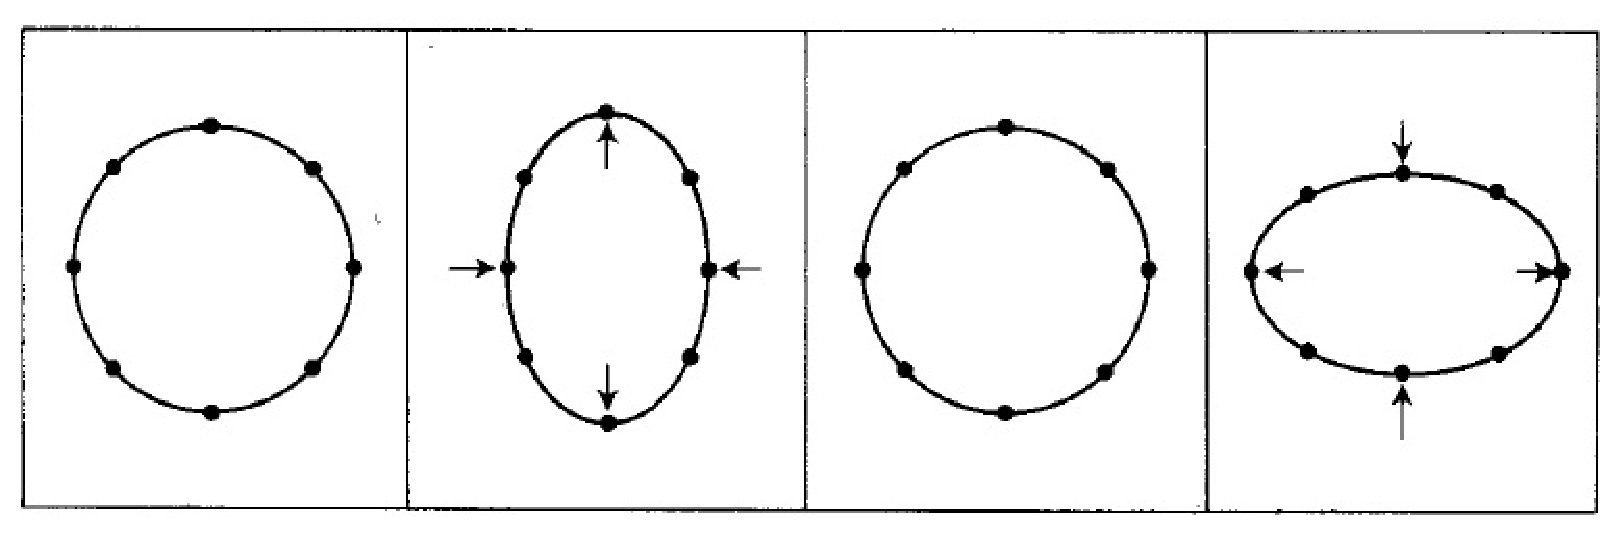
\includegraphics[width=0.5\linewidth]{figures/Introduction/pluspol.eps}
  \caption{Effect of plus ($+$) polarisation}
  \label{fig:sub1}
\end{subfigure}\\
\begin{subfigure}{\textwidth}
  \centering
  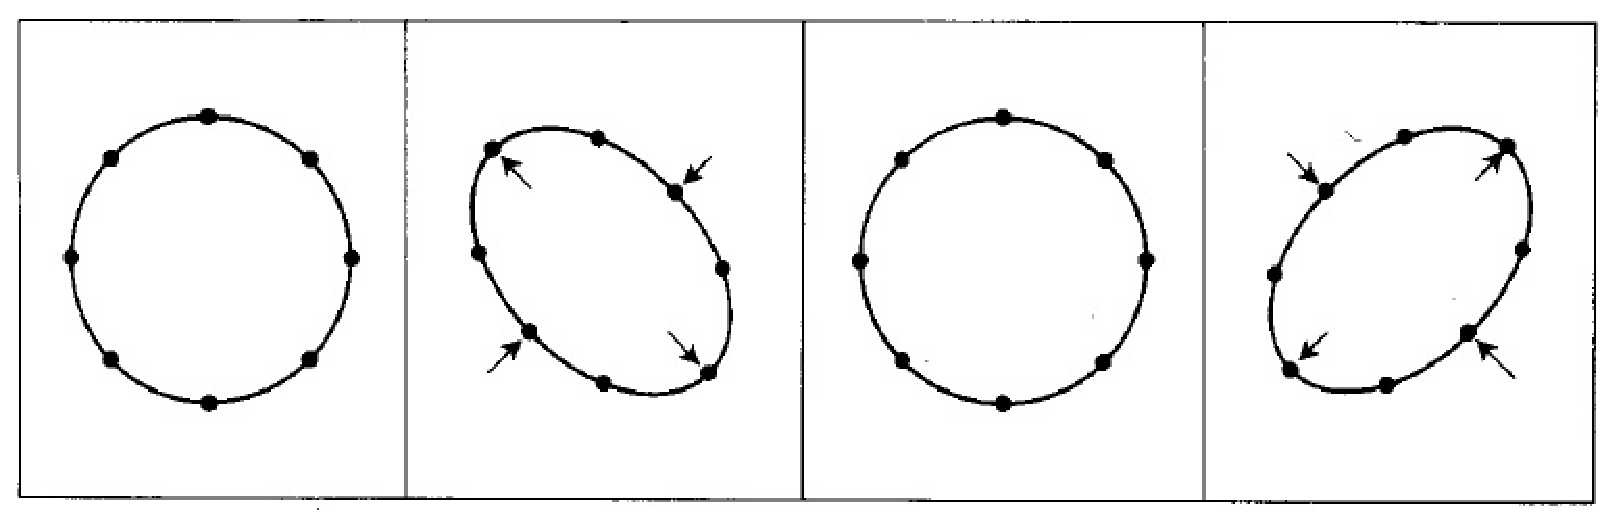
\includegraphics[width=0.5\linewidth]{figures/Introduction/crosspol.eps}
  \caption{Effect of cross ($\times$) polarisation}
  \label{fig:sub2}
\end{subfigure}
\caption{Effect of gravitational waves as it passes through a ring of freely falling particles in the $x-y$ plane (from left to right). The GW is perpendicular into the paper. GWs affect the proper distances between the particles -- effects are shown independently for a wave with the plus (top), and cross (bottom) polarization. For the plus polarization, the circle stretches in $x-$direction and squeezes in $y-$direction simultaneously. Similar pattern for the cross polarization is observed along the diagonals.}
 %The effect of an oscillatory linear plane GW with (a) plus (top) and (b) cross polarisation (bottom) on a ring of freely falling particles. The GW is perpendicular to the paper.}
\label{fig:Polarisation}
\end{figure}



\subsection{Gravitational-wave emission in linearized gravity}
Until now we have discussed the propagation of gravitational waves without discussing how they are generated. In this subsection, we discuss the generation of GWs using the linearized Einstein's equations to a leading order -- we show these waves are a result of the quadrupole radiation. For this purpose, we follow the derivation in \cite{Maggiore:2008aaa}, and refer the reader to the text for more details. 

We revisit the Einstein's equations in the weak-field limit $\Box \bar{h}_{\mu\nu} = -16\pi T_{\mu\nu}$. Considering the source to be at the origin and an observer at the position $\vec{x}'$. As shown in \cite{Maggiore:2008aaa}, the solution to the Einstein's equations can be obtained using the Green's function,
\begin{align}
    \bar{h}_{\mu\nu}(t, \vec{x}) = 4 \int d^3x' \dfrac{T_{\mu\nu}(t-\norm{\vec{x}-\vec{x}'},\vec{x}')}{\norm{\vec{x}-\vec{x}'}}.
    \label{Eq:EQ-greens-function}
\end{align}
We can then approximate the GW emission using the quadrupole emission, using two assumptions -- the observer is far away ($\norm{\vec{x}-\vec{x}'} \approx \norm{\vec{x}} = r$) and the source velocity is small compared to the speed of light.  Under the quadrupolar approximation, Eq. (\ref{Eq:EQ-greens-function}) simplifies to
\begin{align}
    \bar{h}_{\mu\nu}(t, \vec{x}) = \dfrac{4}{r} \int d^3x' T_{\mu\nu}(t-r,\vec{x}').
    \label{Eq:Far-field-greens}
\end{align}

It is easier to compute the above equation by projecting into the TT gauge. Using the laws of conservation of total energy and momentum, the right-hand side of the above equation can be written as 
\begin{align}
    \dfrac{4}{r} \int T_{\mu\nu} d^3x' = \dfrac{2}{r} \dfrac{\partial^2}{\partial t^2} \int T_{00} x_{\mu}x_{\nu} d^3x',
    \label{Eq:before-quadrupole-tensor}
\end{align}
where $T_{00} \approx \rho$ is the Newtonian mass density. The right-hand side of the Eq. (\ref{Eq:before-quadrupole-tensor}) is referred as the \textit{mass quadrupole moment tensor} of the mass distribution,
\begin{align}
    I_{\mu\nu} := \int T_{00}x_{\mu}x_{\nu}d^3x'.
    \label{Eq:quadrupole-tensor-def}
\end{align}
Substituting Eq. (\ref{Eq:quadrupole-tensor-def}) in (\ref{Eq:Far-field-greens}) gives the \textit{quadrupole formula}
\begin{align}
    h_{\mu\nu}^{TT} = \dfrac{2}{r}\ddot{I}_{\mu\nu}^{TT}(t-r),
    \label{Eq:second-order-metric-perturb}
\end{align}
where the $\ddot{I}_{\mu\nu}^{TT}$ represents the second order time derivative of the quadruple moment tensor with the retarded time $(t-r)$ due to the travel time from the source to the observer at a distance $r$. 

By the conservation of energy, the total power radiated by a source must be same as the energy carried by the gravitational waves. The total power radiated by a source is the luminosity flux, which can be obtained by integrating the energy flux over a sphere with infinite radius. Using an analog for the energy-momentum tensor in terms of $h_{\mu\nu}$, we can write the following equations
\begin{align}
    &\dfrac{dE}{dt} = -\mathcal{L}.
    \label{Eq:energy-equation}
\end{align}
The flux $\mathcal{L}$  at a large distance from the source is given as \cite{Peters:1964zz}
\begin{align}
    \mathcal{L} = \dfrac{1}{5}\overline{\dfrac{d^3Q^{jk}}{dt^3}\dfrac{d^3Q_{jk}}{dt^3}} \hspace{0.5cm} \text{and} \hspace{0.5cm} Q_{jk}(t) = \int \rho(t,x^i)\Big(x_jx_k -\dfrac{1}{3}\delta_{jk}x^lx_l \Big)d^3x,
    \label{Eq:flux-equation}
\end{align}
where the bar on top represents an average in all directions, $\rho$ is the mass distribution and $\delta_{ij}$ is the Kronecker symbol. Thus, any source with non-vanishing second derivative of the mass quadrupole moment will emit GWs. Below we outline a few astrophysical sources that are likely to generate strong GWs detectable by current or future observatories. 

\subsubsection{Astrophysical sources of gravitational radiation}
Four primary types of sources are anticipated to produce gravitational emissions strong enough to be detected by existing or proposed GW observatories in the foreseeable future:  
\begin{itemize}
\item \underline{\textit{Compact binary mergers}}: The primary focus of this thesis, these sources are comprised of two compact objects such as black holes or neutron stars, orbiting each other in close proximity. As they orbit, the component objects accelerate and produce gravitational waves. The energy carried away by the GWs leads to a gradual dissipation of the system's orbital energy. This process, unfolding over thousands of millennia, results in a progressively diminishing distance between the objects. As the separation between orbiting objects decreases, their orbital velocities increases, enhancing GW emissions. This results in faster energy loss and an accelerated reduction in their distance \cite{Peters:1963ux,Peters:1964zz}. This relentless progression ultimately binds the objects in an irreversible, accelerating spiral, driving them towards an inevitable merger. Compact binary mergers can be classified by the type of component objects involved, into three types: Binary Black Holes (BBH), Binary Neutron Stars (BNS), and Neutron Star – Black Hole Binaries (NSBH). Additionally, they can be categorized by orbital characteristics (such as circular or eccentric orbits) or the spins of the involved components. As of the drafting of this thesis, compact binary systems are the only confirmed sources of gravitational waves (GWs). Observations of these sources will be detailed in the following chapter.

%Binary Black Holes (BBH): BBH mergers involve two black holes spiraling inwards and merging. The post-Newtonian formalism, which provides a series expansion in terms of the velocity of the objects divided by the speed of light, can be used to describe the inspiral phase. For the merger and ringdown phases, numerical relativity simulations are required, as the gravitational fields are extremely strong and the dynamics are highly nonlinear.

%Binary Neutron Stars (BNS): BNS mergers involve two neutron stars. In addition to the gravitational-wave emission, these events can also result in electromagnetic signals, such as gamma-ray bursts. The inspiral can be modeled using post-Newtonian formalism, but tidal effects (which are important for neutron stars) must also be taken into account. Numerical relativity simulations are required to accurately model the merger and post-merger phases, including the potential formation of a hypermassive neutron star or a black hole.

%Neutron Star – Black Hole Binaries (NSBH): These binaries involve a neutron star and a black hole. The modeling of these systems is similar to BNS mergers, but with additional complexity due to the interaction of the neutron star with the black hole’s tidal field, which can lead to the disruption of the neutron star.

\item \underline{\textit{Periodic sources}}: Compact objects such as spinning neutron stars could have deviations from the perfect axis-symmetric configurations due to deformations induced by: strong magnetic fields \cite{Chandrasekhar:1953zz}, or matter accretion can exhibit features like mountains or deformations on their crusts \cite{Brown:1997ji,Bildsten:1998ey}. Such sources continuously emit gravitational-waves which are near-monochromatic over long time scales \cite{Thorne:1980ru}, and these signals are called as continuous-wave (CW) signals. The predicted and measured constraints on the amplitudes of CW signals is $\sim 10^{-3}$ weaker than the observed compact binary signals. Finding these long duration, incredibly weaker CW signals is an ongoing effort (see \cite{Riles:2022wwz} for a review on CW searches), but they remain elusive to detection by the current GW observatories \cite{Pagliaro:2023bvi}. 

\item \underline{\textit{Burst}}:   In the final evolutionary stages of a massive star, the core of the star implodes and then explodes, releasing a massive shock wave - this explosion is called as a core-collapse supernovae. Gravitational radiation arises from these explosions unless they exhibit perfect spherical symmetry \cite{Abdikamalov:2020jzn}. The precise process underlying supernovae remains incompletely understood, making it challenging to accurately model the gravitational radiation they emit \cite{Abdikamalov:2020jzn, Janka:2012wk}.

\item \underline{\textit{Stochastic background}}: A stochastic background of gravitational-waves will emerge from the cumulative, incoherent superposition of numerous undetected gravitational-wave signals. The source of stochastic gravitational background could be of cosmological origin such as from the inflationary epoch \cite{Barnaby:2011qe}, early universe phase transitions \cite{Hindmarsh:2015qta} or alternate cosmological theories \cite{Buonanno:1996xc}. On the other hand, an astrophysical cosmological background could also exist, potentially arising from GW events such as supernovae, spinning neutron stars or mergers of neutron stars or black holes throughout the universe's history. Recent observations \cite{Reardon:2023gzh,NANOGrav:2023hde,EPTA:2023fyk,Xu:2023wog} from the Pulsar Timing Array (PTA) community has shown evidence for a nano-Hertz stochastic GW background signal \cite{Hellings:1983fr}, whose origins remain elusive. 

%Signals from numerous randomly independent and varied gravitational sources superimpose to form "stochastic signal".  

%The stochastic background of gravitational radiation constitutes a fundamental cosmic signal, emerging from the superposed gravitational-waves produced by an array of astrophysical sources throughout the universe. This omnipresent background is theorized to be the cumulative result of numerous independent and varied cosmic events, ranging from binary mergers of black holes and neutron stars to primordial processes in the nascent universe. Additionally, it potentially includes contributions from yet-to-be-elucidated astronomical phenomena. This amalgamation of gravitational-waves from disparate origins results in a continuous, non-directional background noise, offering a unique probe into both the specific astrophysical events contributing to it and the broader evolution and structure of the universe
\end{itemize}


%\begin{align}
%    &\dfrac{dE}{dt} = -\mathcal{L}, \\
%    &\dfrac{dv}{dt} = -\dfrac{\mathcal{L}}{dE/dv},
%\end{align}
%with the flux $\mathcal{L}$ given as
%\begin{align}
%    \mathcal{L} = \dfrac{1}{5}\overline{\dfrac{d^3Q^{jk}}{dt^3}\dfrac{d^3Q_{jk}}{dt^3}} \hspace{0.5cm} \text{and} \hspace{0.5cm} Q_{jk}(t) = \int \rho(t,x^i)\Big(x_jx_k -\dfrac{1}{3}\delta_{jk}x^lx_l \Big)d^3x,
%\end{align}
%where $\rho$ is the mass distribution and $\delta_{ij}$ is the Kronecker symbol. 


\section{Modeling Compact Binary Mergers}
This section outlines a framework of modeling GWs from compact binary mergers. First, we describe GWs (at leading quadrupole order) for simple binary systems with point-like masses using the Newtonian formalism. Subsequently, we touch upon the Post-Newtonian approach, which offers a more comprehensive depiction of realistic systems. Concluding the section, we provide an overview of different waveform models that effectively represent the entire GW signal, spanning from the inspiral phase of the merging objects to the final phase, marked by the ringdown of the merged remnant.

Compact binaries can be characterized by 19 parameters as listed in the Table \ref{tab:CBC-params}. These parameters are broadly categorized based on the intrinsic properties of the source and the extrinsic properties relating to an observer (detector): 
\begin{itemize}
    \item \underline{Intrinsic parameters}: 
    \begin{itemize}
        \item Component masses ($m_1, m_2$), typically $m_1 \geq m_2$.
        \item Dimensionless component spin vectors ($\vec{\chi}_1, \vec{\chi}_2$).
        \item The amount of deformation of the two compact objects in the vicinity to an external field \cite{Hinderer:2007mb}, denoted as the tidal deformability parameters $\Lambda_1, \Lambda_2$ (note, $\Lambda$ for black holes is assumed to be zero in GR). We ignore these parameters in this thesis.
        \item The orbital eccentricity $e$ defined at a reference orbital frequency.
    \end{itemize}
    \item \underline{Extrinsic parameters}:
    \begin{itemize}
        \item The sky position of the source is given by two angles $(\alpha, \delta)$ called as the right-ascension and declination respectively.
        \item Luminosity distance to the source $d_L$.
        \item Orientation of the binary plane in terms of the inclination angle $\iota$, which is defined as the angle between the orbital angular momentum vector \textbf{L} and the line of sight vector $N$.
        \item Polarization angle $\psi$ required to define the orientation of the effect on a ring of particles by the GW radiation.
        \item An additional angle to describe the perigee of an eccentric orbit which is defined in terms of an unphysical angle called the mean anomaly parameter $l$ (see Fig. \ref{fig:ecc-angles}).
        \item  The time and orbital phase at coalescence denoted as $(t_c, \Phi_c)$ respectively.
    \end{itemize}  
\end{itemize}
The various angles can be visualized with the help of the figures \ref{fig:gw-ref-frame} and 
\ref{fig:ecc-angles}.

\begin{table}[h]
    \centering
    \begin{tabular}{cc}
       Binary parameters   & Symbols\\ \hline
       Component masses  & $(m_1, m_2)$\\
       Component spin vectors    & $(\vec{\chi}_1, \vec{\chi}_2)$\\
       Sky location of the source  & $(\alpha, \delta)$ \\
       Luminosity distance to the source  & $d_L$ \\
       Inclination angle  & $\iota$ \\
       Coalescence phase  & $\Phi_c$ \\
       Polarization angle  & $\psi$ \\
       Coalescence time of the signal at the detector & $t_c$ \\
       Eccentricity and mean anomaly  & $(e, l)$\\
       Tidal deformabilities & ($\Lambda_1, \Lambda_2$)\\  \hline 
    \end{tabular}
    \caption{List of 19 parameters to describe a generic compact binary system. See Fig. (\ref{fig:gw-ref-frame}) and (\ref{fig:ecc-angles}) for visualizations of the mentioned angles.}
    \label{tab:CBC-params}
\end{table}

\begin{figure}
    \centering
    \includegraphics[width=\textwidth]{figures/Introduction/gw-ref-frame.png}
    \caption{Diagram showing the various parameters required to characterize the GW signal from a compact binary merger (see Table \ref{tab:CBC-params} for the complete list). Three different frame of reference are used to map the signal from the source to the observer. First, is the source frame (in red) defined as the plane parallel to the orbital plane with the orbital angular momentum along the frame's $z-$axis. The GW emission in the direction of the observer is then projected on to the radiation frame (this plane is equivalent to the plane of hypothetical ring of test particles). Finally, the GW radiation will be projected in the sky as a tangent plane on a sphere -- this is the detector frame (orange), whose position is described by two sky angles ($\alpha, \delta$). Image was inspired from Fig. 3.5 of \cite{Schafer:2023pbm}.}
    \label{fig:gw-ref-frame}
\end{figure}

\subsection{Point mass particles in Keplerian orbits}\label{sec:circular-binary-PN}  
In this subsection, we outline the key steps to obtain the gravitational waveform for a simple system with point-like masses in circular orbit (with decaying radius) not close to merging. Additionally, we briefly examine the frequency spectrum of the waveform for this case. We then extend our discussion to systems with eccentric orbits or spinning components and highlight the key features in their evolution.

\subsubsection{Quasi-circular binary}\label{sec:circular-binary}
For demonstration, we assume two point objects with masses ($m_1, m_2$) in a quasi circular orbital decay, which is equivalent to the formulation of the Kepler two body problem for a circular orbit 
\begin{align}
    v^2 = \dfrac{M}{d}, \hspace{2cm} \omega_{\text{orbit}} = \sqrt{\dfrac{M}{d^3}} = \dfrac{d\Phi_{\text{orbit}}}{dt},
\end{align}
where $M = m_1 + m_2$ is the total mass of the system, $d$ is the separation between the two particles, $v$ is the relative velocity and ($\omega_{\text{orbit}}, \Phi_{\text{orbit}}$) are the orbital frequency and orbital phase respectively. Choosing a frame of reference with the binary plane equal to the $x-y$ plane, with the binary situated at a distance $d_L$ from the origin (observer), the metric perturbation Eq. (\ref{Eq:second-order-metric-perturb}) can be derived to be 
\begin{align}
   h_{\mu\nu} = \dfrac{4\mu d^2\omega_{\text{orbit}}^2}{d_L} \begin{bmatrix}
                0 & 0 & 0 & 0 \\
                0 & -\cos(2\omega_{\text{orbit}}t) & -\sin(2\omega_{\text{orbit}}t) & 0 \\
                0 & -\sin(2\omega_{\text{orbit}}t) & \cos(2\omega_{\text{orbit}}t) & 0 \\
                0 & 0 & 0 & 0 
                \end{bmatrix}
    \label{Eq:two-body-h-matrix}
\end{align}
where $\mu = \dfrac{m_1m_2}{m_1+m_2}$ is the reduced mass of the system. The GW radiation is emitted in all directions, but we are interested only in the emission along the line of sight between the source and a detector, defined by the inclination angle $\iota$. Thus, we perform a final projection of Eq. (\ref{Eq:two-body-h-matrix}) to get the waveform polarizations (as depicted in Fig. (\ref{fig:gw-ref-frame}))
\begin{align}
    h_{+}(t) &= \dfrac{4M\eta v^2}{d_L}\Big(\dfrac{1+\cos^2\iota}{2}\Big)\cos(2\omega_{\text{orbit}}t+2\Phi_c), \label{Eq:toymodel-plus}\\
    h_{\times}(t) &= \dfrac{4M\eta v^2}{d_L}\Big(\dfrac{\cos \iota}{2}\Big)\sin(2\omega_{\text{orbit}}t+2\Phi_c) \label{Eq:toymodel-cross}
\end{align}
where $\eta = m_1m_2/M^2$ is the symmetric mass ratio and $\Phi_c$ is the orbital phase of the system at the time of coalescence.  We can define the gravitational-wave phase $\Phi$ as  
\begin{align}
    \Phi = 2\Phi_{\text{orbit}} = \int_{t_0}^{t} \omega_{\text{orbit}} dt,
    \label{Eq:GW-phase-integral-circular}
\end{align}
where $\Phi_{\text{orbit}}$ is the orbital phase, and $t_0$ is the initial time. Notice, the orbital velocity of GWs, $\omega_{\text{GW}} = 2\omega_{\text{orbit}}$ is twice the orbital frequency of the system, this also leads to $f_{\text{GW}} = \omega_{\text{orbit}}/\pi$. This simple relationship is not valid in the case of eccentric orbits \cite{Peters:1964zz}. Therefore, the crux of determining the GW polarizations fundamentally lies in tracking how the orbital phase $\omega_{\text{orbit}}(t)$ over time.

For our simple example, the circular orbit assumption allows us to relate the orbital velocity $\omega_{\text{orbit}}$ with the orbital separation $d$, using the Kepler's law
\begin{align}
    \omega_{\text{orbit}}^2 = M/d^3. 
    \label{Eq:kepler-d-omega}
\end{align}
We introduce a new quantity called the \textit{chirp mass} of a binary system
\begin{align}
    \mathcal{M}_c = \mu^{3/5}M^{2/5} = \dfrac{(m_1m_2)^{3/5}}{M^{1/5}}.
\end{align}
Solving the Eqs. (\ref{Eq:energy-equation}) and (\ref{Eq:flux-equation}), the power radiated by this binary system in a circular orbit (to dominant order) is 
\begin{align}
    \dfrac{dE}{dt} = -\dfrac{32}{5}(\mathcal{M}_c\omega_{\text{orbit}})^{10/3}.
    \label{Eq:circular-orbit-Eloss}
\end{align}
The total energy of the system can be written as
\begin{align}
    E &= -\dfrac{m_1m_2}{2d},\\
    &= - \dfrac{1}{2}(\mathcal{M}_c^5\omega_{\text{orbit}}^2)^{1/8},
\end{align}
substituting this in the Eq. (\ref{Eq:circular-orbit-Eloss}) and solving the differential equation gives the evolution of orbital frequency as a function time 
\begin{align}
    \omega_{\text{orbit}}(t) &= \Big(-\dfrac{256}{5}\mathcal{M}_c^{5/3}(t-t_0) \Big)^{-3/8},\\
    &= \dfrac{1}{8}\Big(\dfrac{\tau}{5}\Big)^{-3/8}\mathcal{M}_c^{-5/8}, \label{Eq:omega_circular} %\label{Eq:omega-circular-newtonian}
\end{align}
where $t_0$ is the fiducial starting time for integration which is used to map the time to define a new time variable $\tau = t_c - t$. Plugging Eq. (\ref{Eq:omega_circular}) into Eq. (\ref{Eq:GW-phase-integral-circular}) and solving the equation yields the GW orbital phase (showing explicit dependence of $G$ and $c$)
\begin{align}
    \Phi(\tau) = -2\Big( \dfrac{5G\mathcal{M}_c}{c^3} \Big)^{-5/8} \tau^{5/8} + 2\Phi_{c},
    \label{Eq:gw-circular-newtonian-phase}
\end{align}
again where $\Phi_c$ is the GW phase at the coalescence. Finally, combining Eqs. (\ref{Eq:omega_circular}), (\ref{Eq:kepler-d-omega}) with Eqs. (\ref{Eq:toymodel-plus}), (\ref{Eq:toymodel-cross}), we get 
\begin{align}
    h_+(\tau) &= \dfrac{1}{d_L}\Big(\dfrac{G\mathcal{M}_c}{c^2}\Big)^{5/4}\Big(\dfrac{5}{c\tau}\Big)^{1/4}\Big(\dfrac{1+\cos^2\iota}{2}\Big)\cos\Phi(\tau),\\ 
    h_{\times}(\tau) &= \dfrac{1}{d_L}\Big(\dfrac{G\mathcal{M}_c}{c^2}\Big)^{5/4}\Big(\dfrac{5}{c\tau}\Big)^{1/4}\cos \iota\sin\Phi(\tau). 
\end{align}
The above equations show both the amplitude and frequency increases as the system approaches the coalescence similar to a bird's  ``chirp", and thus, is known as a \textit{chirp signal}. It is evident from the equations, that at the leading order, the amplitude and phase evolution are dependent only on the chirp mass. \\
%This may not true for more complicated systems such as with eccentric orbits or spinning components.\\

\begin{figure}
    \centering
    \includegraphics[width=\textwidth]{figures/Introduction/newtonian-waveform.png}
    \caption{$h_+$ polarization of the quadrupole GW emission from a binary with component masses $m_{1}=m_2=10M_{\odot}$, face-on at a distance of $500$ Mpc from the observer.}
    \label{fig:newtonian-waveform}
\end{figure}

\noindent\underline{\textit{Fourier transform of the chirp signal}}\\

The Fourier domain provides a straightforward way to identify GW signals and filter noise (as we will discuss in later sections). Thus it is crucial to understand the frequency spectrum of gravitational radiation. Considering a signal of the form $h(t) = A(t)\cos\Phi(t)$ can be approximated using the \textit{stationary phase approximation} (SPA) which provides an estimate of the Fourier transform \cite{Dhurandhar2022-hc}, given by,
\begin{align}
    \tilde{h}(f) \simeq \dfrac{1}{2}A(t)\Big(\dfrac{df}{dt}\Big)^{-1/2}e^{i(2\pi ft - \Phi(f) -\pi/4)}.
    \label{Eq:SPA}
\end{align}
We can write the corresponding expressions for $t(f)$ and $\Phi(f)$ from Eqs. (\ref{Eq:omega_circular}) and (\ref{Eq:gw-circular-newtonian-phase}) 
\begin{align}
    t(f) &= t_c - 5(8\pi f)^{-8/3}\mathcal{M}_c^{-5/3},\\
    \Phi(f) &= \Phi_c - 2(8\pi \mathcal{M}_cf)^{-5/3},
\end{align}
Considering only the plus polarization of the chirp signal, we substitute the above equations in the Eq. (\ref{Eq:SPA}), we get the Fourier transform of the Newtonian chirp signal (see \cite{Dhurandhar2022-hc} for the derivation)
\begin{align}
    \tilde{h}(t_c;f) = \sqrt{\dfrac{5}{24}} \dfrac{G^2\mathcal{M}^2_c}{c^5d_L}\Big(\dfrac{\pi G\mathcal{M}_cf}{c^3} \Big)^{-7/6} \Big( \dfrac{1+\cos^2\iota}{2}\Big) e^{i\Phi(f;t_c)},
\end{align}
where
\begin{align}
    \Phi(t_c;f) = \dfrac{\pi}{4} - \dfrac{3}{128}\Big(\dfrac{\pi G\mathcal{M}_cf}{c^3}\Big)^{-5/3} - 2\pi ift_c + \Phi_c.
\end{align}


%The GW polarizations for a circular binary depend on the trignometric functions of their orbital phase (Eqs. (\ref{Eq:toymodel-plus}), (\ref{Eq:toymodel-cross})). However, in case of eccentric orbits this phase becomes a complex function of the orbital frequency -- the phase is related to the arctangent of the eccentric anomaly (Eq. \ref{Eq:true-anomaly}), which is further related to the mean anomaly (Eq. \ref{Eq:ecc-kepler-eq}). The orbital phase $\Phi$ can be written in terms of the eccentricity and Bessel functions with mean anomaly as the argument (see the Appendix \cite{MorenoGarrido1994} for explicit equations).



\subsubsection{Evolution of binary system with eccentric orbits}

The system described earlier can be expanded to include eccentric binary systems in Keplerian orbits. Here, we discuss only the evolution of the eccentric orbits and not the GW polarizations by following the derivations in \cite{Peters:1963ux,Peters:1964zz}.

By adopting the center-of-mass frame, positioned at a focal point of an ellipse, we can describe the binary as a single-body problem with mass $\mu = m_1m_2/M$ moving in an elliptical orbit with semi-major axis $a$, as shown in the Fig. (\ref{fig:ecc-angles}). The angle $\nu$ swept by the body since the perigee ($x-$axis) is called as the \textit{true anomaly}. We also consider an auxiliary circle of radius $a$ to describe two new angles -- 1) the angle between the projection of the body on the circle and the $x-$axis, is the \textit{eccentric anomaly} $u$, and, 2) a hypothetical angle, called the \textit{mean anomaly}, that changes with a constant rate of $2\pi/T$ where $T$ is the time required by the body to complete one eccentric orbit. The parameterized equations of the elliptical trajectories are 
\begin{align}
    d &= a(1 - e\cos u), \\
    \Phi - \Phi_c &= \nu = 2\arctan\Bigg( \sqrt{\dfrac{1+e}{1-e}\tan\dfrac{u}{2}}\Bigg), \label{Eq:true-anomaly}
\end{align}
where $e$ is the eccentricity parameter, $d$ is the distance of the body to the center-of-mass. The Kepler equation relating the two new angles to the mean anomaly $l$ is given by
\begin{align}
    l = u - e\sin u. \label{Eq:ecc-kepler-eq}
\end{align}
And the angular velocity is given by 
\begin{align}
    \dot{\nu} = \dfrac{\sqrt{Ma(1-e^2)}}{d^2}.
\end{align}

\begin{figure}
    \centering
    \includegraphics[width=0.6\textwidth]{figures/Introduction/ecc-angles.png}
    \caption{A reduced mass object in an eccentric Keplerian orbit (blue) with semi-major and minor axis ($a,b$) respectively and with the center of mass (C.O.M) at one of the foci. The angle swept by the reduced mass from the perigee ($x-$axis) is the true anomaly $\nu$. We define two more angles using a hypothetical auxiliary circle with the same radius as the semi-major axis ($a$). The angle between the object's projection onto the circle and the $x-$axis is referred as the eccentric anomaly ($u$). If the object takes $T$ time to finish one eccentric orbit, then the angle changing at a constant rate $2\pi/T$ is defined as the mean anomaly $l$.}
    \label{fig:ecc-angles}
\end{figure}


The orbital parameters $a$ and $e$ are not constants of motion, and will vary over time due to the energy loss via GW emission. Following \cite{Peters:1963ux}, these parameters can be related to the rate of energy emitted by the system averaged over one eccentric cycle  
\begin{align}
    \langle \dfrac{dE}{dt} \rangle = -\dfrac{32}{5}\dfrac{G^4}{c^5}\dfrac{m_1^2m_2^2M}{a^5}\underbrace{\dfrac{1}{(1-e^2)^{7/2}}\Bigg(1 + \dfrac{73}{24}e^2 + \dfrac{37}{96}e^4 \Bigg)}_{f(e)},
    \label{Eq:energy-evol}
\end{align}
which is the average power emitted by a circular binary multiplied by the enhancement factor  $f(e)$. For example, for the Hulse-Taylor binary pulsar with $e \simeq 0.617$, resulting in $f(e) \simeq 11.8$, an order of magnitude larger power is emitted compared to the same system in circular orbit.

Similarly, one obtains the differential equation for the average rate of angular momentum $L = \mu d^2\dot{\nu}$ emission
\begin{align}
    \langle \dfrac{dL}{dt} \rangle = \dfrac{32}{5}\dfrac{G^{7/2}}{c^5}\dfrac{m_1^2m_2^2M^{1/2}}{a^{7/2}(1-e^2)^{2}}\Bigg(1 + \dfrac{7}{8}e^2 \Bigg).
    \label{Eq:angmomentum-evol}
\end{align}

Using Eqs. (\ref{Eq:energy-evol}) and (\ref{Eq:angmomentum-evol}), one can derive equations for the average rate of loss for the semi-major axis $\langle da/dt \rangle$ and eccentricity $\langle de/dt \rangle$
\begin{align}
    \langle \dfrac{da}{dt} \rangle = -\dfrac{64}{5}\dfrac{G^3m_1m_2M}{c^5a^3(1-e^2)^{7/2}}\Big(1+\dfrac{73}{24}e^2+\dfrac{37}{96}e^4\Big), \label{Eq:da-dt} \\
    \langle \dfrac{de}{dt} \rangle = -\dfrac{304}{15}\dfrac{G^3m_1m_2M}{c^5a^4(1-e^2)^{5/2}}e\Big( 1+\dfrac{121}{304}e^2\Big). \label{Eq:de-dt}
\end{align}
Dividing the above two equations we get the differential equation $\langle da/de \rangle$, which can be solved to obtain 
\begin{align}
    a(e) = \dfrac{c_0 e^{12/19}}{(1-e^2)}\Big( 1 + \dfrac{121}{304}e^2 \Big)^{870/2299},
    \label{Eq:a-e-relationship}
\end{align}
where $c_0$ is obtained from fixing $a=a_0$ when $e=e_0$. Using Eq. (\ref{Eq:a-e-relationship}), we can uniquely predict the orbital evolution given the initial conditions of the system ($a_0, e_0$). Substituting Eq. (\ref{Eq:a-e-relationship}) in (\ref{Eq:de-dt}), gives the explicit differential equation for the decay of eccentricity  
\begin{align}
    \langle \dfrac{de}{dt} \rangle = -\dfrac{304}{15} \dfrac{G^3m_1m_2M}{c^5c_0^4}\dfrac{e^{-29/19}(1-e^2)^{3/2}}{[1+(121/304)e^2]^{1181/2299}}.
\end{align}
%From the above equation we can infer that systems with larger 

Integrating the above equation, we can estimate the lifetime of the binary with initial conditions ($a_0, e_0$), which is given by 
\begin{align}
    T(a_0, e_0) = \dfrac{15}{304}\dfrac{c_0^4c^5}{G^3m_1 m_2M} \int_0^{e_0} \dfrac{e^{29/19}(1 + (121/304)e^2)^{1181/2299}}{(1-e^2)^{3/2}}de.
    \label{Eq:Decay-time-binary}
\end{align}
The above equation indicate that for a fixed initial orbital separation and total mass of the system, binaries with larger eccentricity merge quicker and radiate away their eccentricity rapidly. By the time the gravitational wave frequency emitted from a binary system reaches the sensitive band of current detectors $\sim 10$ Hz the system will have negligible eccentricities \cite{Belczynski:2001uc}. These estimates are derived assuming the binary source is evolving under no external influence and is emitting energy only via GW radiation. However, measurement of non-negligible eccentricity would hint at alternate evolutionary pathways, and thus, makes orbital eccentricity an important feature of a binary's formation history.      

\subsection{Post-Newtonian treatment}\label{sec:PN-formalism}

We now examine a more realistic scenario where the binary system influences spacetime curvature, moving beyond the flat spacetime model. In this case, Newtonian gravity is insufficient to explain the system's dynamics, necessitating the use of Post-Newtonian (PN) formalism. The PN theory hinges on two primary assumptions: firstly, the sources must move slowly, mirroring the requirement of linearized theory where $v/c$ is much less than one. For relativistic objects, this means including higher-order expansions, beyond the quadrupole. Secondly, the sources should be weakly self-gravitating, meaning the spacetime curvature they create isn't excessively strong. Consequently, the PN formalism is accurate only when the two objects are adequately distant from each other -- only for the inspiral phase.  Assuming the orbital frequency remains almost constant over one cycle, which is the condition for an \textit{adiabatic inspiral}, we can write
\begin{align}
    \omega_{\text{orbit}} = \dfrac{d\Phi_{\text{orbit}}(t)}{dt} = \dfrac{v^3}{M},
    \label{Eq:adiabatic-inspiral}
\end{align}

Several approaches could be used to perform the PN expansions \cite{Will:1996zj,Schafer:2018kuf,Blanchet:2013haa}. Higher-order corrections to the quadrupole GW emission is done in terms of the expansion parameter 
\begin{align}
    x &:= \Big(\dfrac{GM\omega_{\text{orbit}}}{c^3}\Big)^{2/3}, \label{Eq:PN-parameter} \\
    & \propto \mathcal{O}\Big( \dfrac{v}{c} \Big)^2.\notag
\end{align}

The starting point of PN expansion is to obtain the equations of motion as powers of $x^{1/2}$ to the appropriate $n^{\text{th}}$ PN order. Then, expressions for the energy of the orbit and the flux of the source are corrected to the same PN order. For instance, the energy of the orbit up to 3.5 PN order is given as \cite{Maggiore:2008aaa}
\begin{align}
    E(x) = & -\dfrac{\eta Mc^2x}{2}\left\{1 + \Big(-\dfrac{3}{4} - \dfrac{1}{12}\Big)x + \Big( -\dfrac{27}{8} + \dfrac{19}{8}\eta - \dfrac{1}{24}\eta^2 \Big)x^2 \right. \notag \\
    & \left. + \Big[ -\dfrac{675}{64} + \Big(\dfrac{34445}{576} - \dfrac{205}{96}\pi^2\Big)\eta -\dfrac{155}{96}\eta^2 -\dfrac{35}{5184}\eta^3 \Big] \right\} \notag \\
    & + \mathcal{O}\Big(\dfrac{1}{c^8}\Big).
    \label{Eq:energy-3.5PN}
\end{align}
The expression for the flux $\mathcal{L}(x)$ to 3.5 PN order is given in the Eq. (5.257) \cite{Maggiore:2008aaa}.



Combining the energy and flux equations by applying the chain rule energy-flux relation, gives the ordinary differential equation for $dx/dt$  
\begin{align}
    \dfrac{dE}{dt} &= \dfrac{dE}{dx}\dfrac{dx}{dt} = -\mathcal{L}(x), \\
    \Rightarrow \dfrac{dx}{dt} &= -\dfrac{\mathcal{L}(x)}{dE/dx}. \label{Eq:flux-energy-relation}
\end{align}
The loss in energy by the system is the power emitted as GWs. Solving the above equations, one obtains the expression for orbital phase $\Phi_{\text{orbit}}(t)$, which is plugged in the $h_{+,\times}$ polarizations to get the PN waveform \cite{Blanchet:2013haa}.  

Different strategies can be used to solve Eq. (\ref{Eq:flux-energy-relation}), each resulting to different variants of the time domian PN waveform \textit{approximants} --  \approximant{TaylorT1} to \approximant{TaylorT4}. For instance, the \approximant{TaylorT1} approximant \cite{Blanchet:2004ek} solves the Eq. (\ref{Eq:flux-energy-relation}) in terms of $v$ as the expansion parameter -- numerical integration gives $v(t)$, which is again integrated after substitution (Eq. (\ref{Eq:adiabatic-inspiral})) to obtain $\Phi_{\text{orbit}}(t)$. We refer the reader to \cite{Buonanno:2009zt} for a review on the technical details to build these approximants. 

%in terms of the expansion parameter (see Eq. 318 in \cite{Blanchet:2013haa}). Relating the orbital phase with the GW phase, and the expansion parameter with time, gives $\Phi(t)$.  then obtained using and plugged into the waveform polarizations $h_{+,\times}$ (Eqs. 320-323 in \cite{Blanchet:2013haa}).   



\subsubsection{Harmonic structure of gravitational radiation}\label{sec:HMs-sec}
Following the procedure described in subsection \ref{sec:circular-binary-PN}, after obtaining $\Phi_{\text{orbit}}(t)$ and $A(t)$ for a waveform in the source frame, the waveform is then transformed to the radiation frame. This transformation can be described in general as the decomposition of a waveform in terms of spin-weighted spherical harmonics -- representing a set of basis functions on sphere $Y_{lm}^{-s}$ defined as \cite{Brown:2007jx}
\begin{align}
    Y_{lm}^{-s}(\iota,\Phi_c) = (-1)^{s}\sqrt{\dfrac{2l+1}{4\pi}}d^{l}_{ms}(\iota)e^{im\Phi_c},
\end{align}
where $d^{s}_{lm}$ is the Wigner matrix and ($\iota, \Phi_{c}$) are the inclination $\iota$ and the phase at coalescence $\Phi_c$ of the binary w.r.t a given observer. For reference,
\begin{align}
    Y_{2,2}^{-2} = \sqrt{\dfrac{5}{64\pi}}(1+\cos\iota)^2e^{2i\Phi_c}, \hspace{1cm} Y_{2,-2}^{-2} = \sqrt{\dfrac{5}{64\pi}}(1-\cos \iota)^2e^{-2i\Phi_c}
\end{align}

We can now decompose the GW in terms of the spin-2 weighted spherical harmonics as
\begin{align}
    h(t;\iota, \Phi_c) = h_{+} - ih_{\times} = \sum_{l=2}^{\infty} \sum_{m=-l}^{l} h_{lm}(t)Y_{lm}^{-s}(\iota, \Phi_c).
\end{align}
where $h_{lm}$ are the various \textit{modes} of the GW signal which have different contributions to the observed signal via the $Y_{l,m}^{-2}$.  For now, we are interested in the quadrupole emission with $(l,m) = (2,2)$, which is the strongest when the binary is face-on ($\iota = 0$) or edge-on ($\iota = \pi/2$)  and grows fainter with increasing $\iota$ reaching minimum at $\iota = \pi/2$. We combine the above equations to find  
\begin{align}
    h(t;\iota,\Phi_c) &= h_{2,2}(t)Y_{2,2}^{-2}(\iota,\Phi_c) + h_{2,-2}(t)Y_{2,-2}^{-2}(\iota,\Phi_c),\\
    &= A_{2,2}\sqrt{\dfrac{5}{4\pi}}(1+\cos^2 \iota)\cos(2\Phi_{\text{orbit}}-2\Phi_c) \notag\\
    & \hspace{3cm} - iA_{2,2}\sqrt{\dfrac{5}{4\pi}}\cos \iota\sin(2\Phi_{\text{orbit}}-2\Phi_c),\label{Eq:spharm-quadrupole}
\end{align}
where we use $h_{2,2} = A_{2,2}e^{-2i\Phi_{\text{orbit}}}$, where $\Phi_{\text{orbit}}$ is given by Eq. (\ref{Eq:gw-circular-newtonian-phase}) and invoke $h_{2,2}=(h_{2,-2})^*$. The above equation is similar to the Eqs. (\ref{Eq:toymodel-cross}) and (\ref{Eq:toymodel-plus}), and by comparing them we obtain the leading order amplitude 
\begin{align}
    A_{2,2} = \sqrt{\dfrac{64\pi}{5}} \dfrac{M\eta v^2}{d_L}. 
\end{align}

This decomposition procedure also works for PN approximants where the amplitude and orbital phase are defined at higher-order terms. Thus, we can write the generic expression for a given mode ($l,m$) with given amplitude $A_{lm}$ and orbit $\Phi_{l,m}$ 
\begin{align}
    h_{l,m}(t) = A_{l,m}(t)e^{-i\Phi_{l,m}}.
\end{align}

 
\subsubsection{Quasi-circular binary with spinning components}\label{sec:precessing-sec}

Until now we have discussed systems where the components are not spinning. Now let's consider the case of binaries with spinning components. We denote the spin angular momenta 
\begin{align}
    \textbf{S}_1 &= \vec{\chi}_1 m_1^2 \\
    \textbf{S}_2 &= \vec{\chi}_2 m_2^2.
\end{align}
In the case of aligned-spin systems, the direction of the orbital angular momentum remains fixed and the spin vectors $\textbf{S}_1, \textbf{S}_2$, and $\textbf{L}$ remain parallel. %The aligned-spins do not change the linear relationship between the orbital phases $\Phi = m\Phi_{\text{orbit}}$ but only the rate of inspiral is affected. 
And, for systems with generically oriented spin vectors, the spins of the compact objects can couple with the orbital angular momentum causing spin-precession \cite{Apostolatos:1994mx}. For such systems, the orbital angular momentum $\textbf{L}$ precesses around the nearly fixed total angular momentum $\textbf{J} = \textbf{S}_1 + \textbf{S}_2 + \textbf{L}$; and the inclination angle varies over time. The various spin and orientation angles are shown in the Fig. \ref{fig:precessing_angles}. 

Orbital precession introduces a dependency of orbital frequency $\omega_{\text{orbit}}$ and precession frequency $\omega_{p}$ on the evolution of orbital phase
\begin{align}
    \dfrac{d\Phi_{\text{orbit}}}{dt} = \omega_{\text{orbit}} - \omega_{p}\cos\varrho,
\end{align}
where $\varrho = \hat{\textbf{L}}.\hat{\textbf{J}}$ is defined as the opening angle between the vectors $\textbf{L}$ and $\textbf{J}$, such that $\theta_{JN} = \iota + \varrho$. Precession dynamics cause phase and amplitude modulations to the observed signal that contribute to the PN energy and flux at higher than the quadrupole order \cite{Hannam:2013pra,Pekowsky:2013ska}. The spin effects can be conveniently captured in terms of the in-plane and parallel spin components -- commonly characterized as the two effective parameters \cite{Ajith:2009bn, Schmidt:2014iyl}

\begin{align}
    \chi_{\text{eff}} = \dfrac{1}{M}\Bigg(\dfrac{\textbf{S}_1}{m_1}+\dfrac{\textbf{S}_2}{m_2}\Bigg)\cdot\hat{\textbf{L}}, \label{eq:chi_eff_old}\\
    \chi_{p} = \dfrac{1}{A_1m_1^2}\max\Big(A_1 S_1^{\perp},A_2 S_2^{\perp}\Big), \label{eq:chi_P_old}
\end{align} 

where, $A_1=2+3q/2$ and $A_2 = 2 + 3/(2q)$, $q$ is the mass-ratio $m_1/m_2$, and $S_i^{\perp}$ is the projection of the spins orthogonal to $\textbf{L}$. The $\chi_{\text{eff}}$ parameter gives us a measure of the spin components parallel to $\textbf{L}$. The four in-plane spin components are averaged over a precessing cycle to obtain an effective $\chi_p$ precession parameter.

\begin{figure}
    \centering
    \includegraphics[width=0.6\textwidth]{figures/Introduction/Precessing_angles-new.png}
    \caption{The angular momentum vectors for a precessing binary. The inclination angle $\iota$ is defined as the angle between the orbital angular momentum $\textbf{L}$ and the line of sight to the observer $\textbf{N}$. The angle between $\textbf{J}$ and $\textbf{N}$ is denoted as $\theta_{JN}$. Due to spin-orbit coupling, $\textbf{L}$ and $\textbf{S}$ will precess around the approximately fixed $\textbf{J}$.}
    \label{fig:precessing_angles}
\end{figure}

\subsection{Waveform models}
Until now we have discussed only the inspiral phase of a compact binary merger. But the system continues to emit GWs throughout the merger and after the system has settled in to a newly formed object (BH or NS). The GWs from the final object  resemble those from a struck bell, gradually fading as the object stabilizes -- this final phase is called as the \textit{ringdown}. PN approximants starts to break down near the merger and cannot describe the waveform evolution at the later stages. The pre-merger waveform evolution is crucial for detection because binary systems emit higher power close to merger as the orbital frequency increases rapidly (section (\ref{sec:circular-binary})), and the ringdown phase could be used to perform various tests of General Relativity \cite{Dreyer:2003bv}. 

This subsection summarizes three primary waveform model families, encompassing the entire orbital progression from inspiral to merger to ringdown (IMR) (as shown in Fig. (\ref{fig:full-IMR-wf})). These models integrate numerical relativity (NR) simulations which accurately solve the complex and nonlinear Einstein equations, albeit requiring substantial computational resources. Generating a full waveform for the final orbits and merger of a binary system can take weeks or more \cite{Hannam:2009rd}, making direct use in data analysis impractical. Hence, these models blend precise NR waveforms with analytical or semi-analytical approximations to address this limitation.

\begin{figure}
    \centering
    \includegraphics[width=0.9\textwidth]{figures/Introduction/Full-IMR.png}
    \caption{Evolution of a compact binary merger described in three different phases: 1)Inspiral -- The two object are slowly orbiting each other with decreasing orbital separation as GW radiation is emitted from the system. The inspiral part can be accurately described by Post-Newtonian theory or the Effective One Body approach. 2) Merger -- the two objects merge each other into one compact object. Modeling merger requires solving Einstein's equations numerically. 3) Ringdown -- The final object vibrates, releasing damped sinusoidal GWs that can be modeled using perturbation theory. Image credits: \cite{Antelis:2016icm}}
    \label{fig:full-IMR-wf}
\end{figure}

%Previously in section \ref{sec:PN-formalism}, we discussed PN waveforms that are designed primarily for the inspiral phase, which remain accurate until shortly before the merger \cite{Blanchet:2004ek,Santamaria:2010yb}. However 


\subsubsection{Effective-One-Body (EOB)}
%These models map the two-body problem onto an effective one-body problem (EOB), using results from post-Newtonian theory and numerical relativity. It was initially developed to overcome the limitations of post-Newtonian theory in the highly relativistic regime of binary mergers. 

The effective one-body (EOB) model (introduced in \cite{Buonanno:1998gg}) transforms the problem of a binary system into an equivalent problem of a single test particle moving in an effective external gravitational field, described by an effective Hamiltonian \cite{Buonanno:1998gg,Buonanno:2000ef,Damour:2000we,Damour:2001tu}. This Hamiltonian includes not only the leading-order (Newtonian) terms but also higher-order post-Newtonian corrections in a resummed form of non-polynomial functions \cite{Damour:2008te}. The resummation  performed using techniques like Padé approximations to improve the PN convergence in the strong-field regime (see section 14.1 of \cite{Maggiore:2018aab} for detailed calculations). 

The EOB method surpasses the accuracy of PN theory, yet it exhibits some deviation from the ``exact" solution during the merger phase. This deviation is assessed by comparing with the exact solutions provided by NR. Such comparisons enable the calibration of higher PN coefficients to model the inspiral and merger part of the waveform \cite{Buonanno:2007pf}. Finally, the ringdown part is incorporated by applying perturbation theory, creating a full inspiral-merger-ringdown (IMR) waveform \cite{Damour:2007xr}.

The first full IMR EOB model was developed for non-spinning BBH system \cite{Buonanno:2000ef}, which was then extended to spinning BBHs \cite{Buonanno:2000ef}. The EOB models tuned to NR data are referred as the ``EOBNR" models \cite{Buonanno:2007pf}. There is a wide range of EOBNR versions such as \approximant{SEOBNRv1} \cite{Taracchini:2012ig} (where the ``S" denotes (anti-)aligned spins), each differing based on the features of the waveform they focus on and the specific NR data set employed for calibration. Till date the state-of-art model from the EOB family is \approximant{SEOBNRv5\_PHM} \cite{Ramos-Buades:2023ehm,Pompili:2023tna}, that can describe a spinning, precessing binary including the higher-order modes of the GW emission. In the EOB formalism, binary dynamics are characterized by solving a set of coupled ordinary differential equations to get time-domain solutions then converted to frequency-domain representations for use in searches and parameter estimation. This procedure is be computationally demanding due to the typical requirements of evaluating millions of waveforms. Reduced Order Models (ROM) overcome this problem by building Fourier domain waveforms up to $\mathcal{O}(10^3)$ times faster with acceptable loss in accuracy \cite{Purrer:2015tud}.   


\subsubsection{Phenomenological Models}
Phenomenological models present an alternative to EOB models, addressing key issues like complexity and computational expense, which was first introduced in \cite{Ajith:2007qp}. The fundamental principle of the Phenom models is to employ phenomenological ansatz which are callibrated using NR simulations. These phenomenological models are analytical and constructed directly in the Fourier domain and in the time domain \cite{Estelles:2020twz}, using closed-form expressions dependent on the parameters of the binary system being analyzed. This makes these models rapid and eliminates the need for Fourier transformation during parameter estimation studies. From  (anti-)aligned spinning \approximant{IMRPhenomD} model \cite{Ajith:2009bn}, this family of models has undergone many upgrades. The state-of-art Phenom model \approximant{IMRPhenomXPHM} can accurately model full inspiral-merger-ringdown ``IMR", extreme mass ratios ``X", precessing binaries ``P" and higher-order modes ``HM" \cite{Pratten:2020ceb}.


\subsubsection{Surrogate models}
Currently, there are hundreds of Numerical Relativity (NR) simulations accessible, covering extensive portions of the anticipated parameter space for binary black hole mergers \cite{Boyle:2019kee, Healy:2022wdn}. These simulations produce waveforms that represent the most accurate predictions of the radiation emitted by merging binary systems. NR surrogate models are built by interpolating the NR simulations from various catalogs. Generally, they surpass the accuracy of the aforementioned approximate methods. However, their validity is confined to the specific parameter regions encompassed by the base simulations. The current state-of-art surrogate approximant is the \approximant{NRSur7dq4} \cite{Varma:2019csw}, including seven parameters (6 spins + mass ratio) and is valid only up to mass ratio of four. 


%In summary, compact binary merger waveforms are divided into three main parts: \underline{\textit{Inspiral}}: The phase where the two objects are orbiting each other, gradually coming closer, can be approximated using post-Newtonian theory or effective-one-body formalism. \underline{\textit{Merger}}: The phase where the system is very close to coalescence. PN approximations are no longer valid and thus, this phase requires NR simulations for accurate modeling. \underline{\textit{Ringdown}}: The phase after the merger, where the newly formed object (a black hole or a neutron star) settles into its final state, emitting gravitational waves in the process. The ringdown can be modeled using black hole perturbation theory, specifically using quasi-normal modes.


\section{Formation and evolution mechanisms of compact binaries}

Neutron stars (NS) and black holes (BH) with stellar masses typically emerge from the end stages of massive stars. These massive stars are usually not solitary; they often exist in pairs or in even higher multiplicity systems, with many engaging in interactions with their companions, as illustrated in the works of \cite{Sana:2012px,Moe2017}. The dynamics of these interactions, which significantly shape the destiny and observable traits of the stars—as well as the events they catalyze, like compact binary mergers — are not fully understood.

Using Eq. (\ref{Eq:Decay-time-binary}), the maximum separation $a_{\text{merge}}$, a (circular) binary system with total mass $M$ can have when it forms, to ensure it merges within time period $T$ due to the emission of GWs only, is given by
\begin{align}
    a_{\text{merge}} \lesssim 2.7 R_{\odot} \Bigg( \dfrac{M}{M_{\odot}} \Bigg)^{3/4} \Bigg(\dfrac{T}{14 \text{Gyr}}\Bigg)^{1/4}.
\end{align}
Therefore, for a merger to occur within the 14 billion years of the Universe's existence, a BNS with component masses $(1.4,1.4)M_{\odot}$, needs to be within a distance less than 5$R_{\odot}$ (solar radii). Similarly, a BBH with $(35,35)M_{\odot}$ must be closer than a quarter of an astronomical unit (au) for a merger to take place within the same time-frame.

Massive stars often expand to sizes spanning several au over their lifetimes. The central question in understanding the formation of compact binary mergers is: \textit{How can two compact objects come close enough to merge in a time shorter than the age of the Universe, thus making them observable through gravitational wave (GW) detectors?} The solutions typically proposed fall into two categories as shown in Fig. (\ref{fig:two-broad-channels-cartoon}). One involves leveraging the processes of stellar evolution and mass transfer in an isolated binary system to bridge this proximity gap. The other bypasses this challenge by utilizing dynamic interactions to form binaries already at a close enough distance, allowing gravitational-wave emissions to effectively lead them to merge. In this section we provide a brief overview of the two formation channels, some of the various evolution mechanisms and a few key uncertainties involved in these channels. We refer the reader to two extensive review articles on the formation and evolution of compact binary systems \cite{Postnov:2014tza, Mandel:2021smh}.

\begin{figure}
    \centering
    \includegraphics[width=\textwidth]{figures/Introduction/Two-broad-channels-cartoon.png}
    \caption{Cartoon depicting the two broad formation scenarios for compact binary mergers -- an isolated BBH formation through common envelope (left) and a dynamical BBH formation in star clusters (right). Image credits: \cite{Mapelli:2020vfa}.}
    \label{fig:two-broad-channels-cartoon}
\end{figure}


\subsection{Isolated Binary evolution}

\textbullet{\underline{\textit{Via mass transfer}}}\\

This mechanism typically begins with the evolution of the primary star (more massive), overflowing its Roche lobe (gravitational boundary of binary system within which a star's material is gravitationally bound to a star). This prompts the mass transfer to its lighter companion, leaving behind a naked helium star. The primary star continues to burn its nuclear fuel and eventually undergoes a supernovae explosion to collapse into a compact object.  The binary system might become unbound due to mass loss or the natal kick resulting from asymmetric mass ejection in a supernova. If the binary remains bound, the secondary star eventually expands and starts transferring mass to the primary, now a compact object. This process, combined with the primary's mass loss from earlier mass transfer, stellar winds, and the supernova, often results in the secondary becoming more massive than the primary. As a result, the subsequent mass transfer can not only harden the binary but may also trigger dynamic instability \cite{vandenHeuvel:2017pwp}. This instability can lead to the creation of a common envelope \cite{Paczynski:1993gz} -- a shared envelope of gas surrounding the binary. 

When the primary compact object (NS or BH) enters a common envelope phase with the companion giant star, it orbits within the giant star's envelope alongside the star's core. During this orbit, the compact object experiences significant drag from the envelope, leading to a loss of kinetic energy and an inward spiral. This action heats the envelope, potentially causing  ejection of the envelope. If the envelope isn't ejected, the binary system prematurely merges into a single compact object. However, if the envelope is expelled, the resultant system consists of the primary compact object and the giant's naked core, now much closer due to the spiral-in, with a semi-major axis of just a few solar radii, significantly smaller than initially. 

Should the exposed core collapse into a BH without a strong natal kick, it forms a compact binary system with a short orbital period, potentially merging within the age of the universe. Our current understanding of the common envelope phase, as highlighted in \cite{Fragos:2019box} remains limited. We refer the reader to \cite{Paczynski:1993gz} for a detailed explanation of the common-envelope channel. \\

\textbf{Uncertainties in single stellar evolution} significantly influence various astrophysical processes. The extent of massive stars' expansion during their lifetimes dictates the initiation and consequences of mass transfer \cite{Laplace:2020hum}. Stellar winds determine the stars' final masses and separations \cite{Vink:2016epw}. The effectiveness of tidal coupling affects how orbits become circularized \cite{Zahn:1977mi}. The mass lost in supernovae, along with the resulting natal kicks, influences whether binary systems can survive these stellar explosions \cite{Muller:2020ard, Fryer:2011cx}. \\


\noindent \textbullet{\underline{\textit{Chemically homogeneous evolution and Population III stars}}}\\

To circumvent the challenge of accommodating exceedingly large stars within a compact binary system capable of merging via gravitational-waves, it's essential to inhibit their expansion from the outset. In this context, we explore two potential solutions: effective mixing and an original composition devoid of metals, both of which could impede the expansion of stars to avoid mass transfer during the binary evolution.

1) In the chemical homogeneous evolution channel, both stars in a binary system are assumed to be rapidly rotating. This rapid rotation leads to strong internal mixing of the stellar material. As a result, the stars remain chemically homogeneous throughout their lives, preventing the development of a distinct core-envelope structure that is typical in normal stellar evolution. Such a channel requires massive stars which may evolve into black-holes, resulting in only BBH or NSBH binaries via this channel \cite{Marchant:2017ehn}. 

2) Population III stars, believed to be the first generation of stars formed under pristine conditions after the Big Bang, consisting almost entirely of hydrogen and helium (with no heavier elements (metals)). Population III stars are theorized to have possibly hundreds to thousands of times the mass of the Sun, and very short-lived, lasting only 2–5 million years \cite{Ohkubo:2009ft}. These stars may exhibit less radial expansion compared to metal-rich stars, as suggested by \cite{Marigo:2001pm}. This limited expansion allows the stars to evade mass transfer and various challenges associated with the traditional isolated binary evolution channel.

\textbf{Challenges for chemically homogeneous evolution and population III stars}: The effectiveness of chemical mixing remains in question. Due to limited observational data and difficulties in theoretical modeling, the validity of the various assumptions in the two channels casts doubt. Additionally, the potential for significant stellar expansion might altogether negate these as distinct formation channels.


\subsection{Dynamical Formation}

In dynamical formation channels independently evolved BHs or NSs come together by chance to form compact binaries. This kind of encounters occur in dense environment cluster, where the paths of stars and binary stars are frequently disrupted by dynamic encounters with other stars in the cluster. Dynamical encounters can lead to massive binaries components heavier than $\sim 50 M_{\odot}$ \cite{Gerosa:2017kvu,Rodriguez:2019huv}, which is against the prediction due to pair-instability supernovae \cite{Belczynski:2016jno,Woosley:2016hmi}. Dynamically assembled binaries can have isotropically distributed spin orientations \cite{Rodriguez:2016vmx,Talbot:2017yur} and non-negligible orbital eccentricities \cite{Gondan:2018khr,Rodriguez:2018pss}.

Dynamical formation channels can be categorized into various types depending on the binary environment.\\

\noindent\textbullet{\underline{\textit{Dense star clusters}}}\\

Dynamical formation has been studied for three environments, typically differing in age, location, and composition, which are 

\begin{figure}
\centering
\begin{subfigure}[b]{0.48\textwidth}
  \centering
  \includegraphics[width=\textwidth]{figures/Introduction/messier-15.jpg}
  \caption{Globular cluster: Messier 2}
  \label{fig:globular-cluster}
\end{subfigure}
\hfill
\begin{subfigure}[b]{0.48\textwidth}
  \centering
  \includegraphics[width=\linewidth]{figures/Introduction/NGC-6752-YSC.jpg}
  \caption{Young star cluster: NGC 299}
  \label{fig:YSC}
\end{subfigure}
\\
\begin{subfigure}[b]{0.48\textwidth}
  \centering
  \includegraphics[width=\linewidth]{figures/Introduction/NSC.jpg}
  \caption{Nuclear star cluster of our own Milky Way Galaxy}
  \label{fig:NSC}
\end{subfigure}
\caption{Three categories of dense environments classified based on the age of stars and the location and composition of these clusters w.r.t a host galaxy. Image credits: ESA/Hubble and NASA.}

\label{fig:Dense-environments}
\end{figure}

\begin{itemize}
    \item Globular clusters: These are among the oldest known star clusters, often more than 10 billion years old. Often found in the halo of galaxies and often orbiting the galactic center in a spherical distribution. They typically contain hundreds of thousands to millions of stars, which are densely packed. The stars are usually low in metallicity, indicating their formation early in the universe's history.
    \item Young star clusters: As the name suggests, these clusters are relatively young, ranging from a few million to a few hundred million years old. They are generally found in the spiral arms of galaxies, often in star-forming regions. Young star clusters contain fewer stars than globular clusters, usually in the thousands. These stars tend to be high in metallicity and include many massive, hot, young stars.
    \item Nuclear clusters: These clusters can contain a mix of both old and young stars, and are located at the very centers of galaxies, including the Milky Way. Nuclear star clusters are dense and compact, containing a mix of star populations with various ages and metallicities. They often coexist with or around supermassive black holes.
\end{itemize}

When three stars interact (binary-single interaction) in a \textit{dynamical exchange}, the lighter star is often expelled, leaving the heavier ones paired. Binaries with fast orbits become even tighter as they interact and exchange energy with passing stars. If the conditions are right, these tightened binaries might eventually be dominated by gravitational-waves, provided they aren't ejected from the cluster too soon and there's a sufficient rate of interaction \cite{Ziosi:2014sra, Quinlan:1996vp}.

Additionally, the presence of a central supermassive black hole (SMBH) can trigger mergers through the secular Kozai-Lidov effect \cite{Antonini:2016gqe}. In nuclear clusters, which are more massive than globular clusters, neutron stars (NS), black holes (BHs), and their merger remnants can be retained even if they are given significant velocities at birth or during the merger \cite{Antonini:2018auk}.\\


\noindent\textbullet{\underline{\textit{Hierarchical 3-body systems}}\\

Dynamical scenarios are also promising for hierarchical mergers -- where the compact objects might not always be stellar remnants, instead, they can originate from a prior binary merger. %The detection of the event GW190521, where both masses fall in the high mass-gap (65-120$M_{\odot}$) \cite{Woosley:2016hmi} provides a strong evidence for the exsistence of hierarchical merger. 
In hierarchical triple systems, as reviewed by \cite{Naoz2016}, the inner binary and the wider orbit of a third companion exchange angular momentum. This dynamic can periodically heighten the eccentricity of the inner binary, as described by Lidov (1962) and Kozai (1962) \cite{LIDOV1962719,Kozai:1962zz,Antognini:2015loa}. When the inner binary's eccentricity reaches a high level, gravitational-waves or tides can dissipate energy, potentially leading to the merger of the inner binary \cite{Wen:2002km,Liu:2018nrf}.


The formation of neutron star binaries (BNS or NSBH) systems might be significantly influenced by hierarchical triples, but this depends on the assumed natal supernovae kicks of neutron stars \cite{Hamers:2019oeq}. Considering the triple channel further, there's also the possibility of even more complex systems like quadruples \cite{Vynatheya:2021mgl, Fragione:2020aki}.


\subsubsection{Distinguishing isolated vs dynamical formation scenario}

\resizebox{\textwidth}{!}{
\begin{tabular}
    \centering
    \begin{tabular}{cc}
        %\hline
        Isolated formation & Dynamical formation \\
         \hline
         Spins aligned to the orbital angular momentum & Randomly oriented spins\\
         Negligible eccentricity & Non-negligible eccentricity \\
         Components $60 < M_{\odot}$ (upper mass gap) & Components in the upper mass gap are possible \\
         \hline
         \caption{Summary of the key differences in binary parameters expected from the two broad channels.}
    \end{tabular}
    \label{tab:formation-models-summary}
\end{tabular}
}
\\

Mergers formed dynamically are expected to exhibit characteristics distinct from those arising from isolated binaries, which might help in differentiating their formation processes. For instance, in dynamic mergers, the components evolve independently, leading to randomly oriented spins relative to each other \cite{Rodriguez:2016kxx}. This contrasts with isolated binary systems where spins are typically aligned with the orbital angular momenta, barring disturbances during compact object formation \cite{OShaughnessy:2017eks, Gerosa:2018wbw}. Additionally, interactions in small groups or in dense environments can result in significant eccentricity when binary systems evolve in frequency to the sensitive band of current detectors (i.e. eccentricity $e_{10}$ at 10 Hz): up to 80\% of binary mergers influenced by the LK mechanisms are expected to have $e_{10} \geq 0.01$ in hierarchical triples or nuclear clusters \cite{Hamers:2019oeq, Fragione:2018yrb,Trani:2021tan, Silsbee:2016djf,Rodriguez:2018jqu}, and up to 5\% of mergers in globular clusters are estimated to exhibit $e_{10} \geq 0.1$ \cite{Samsing:2017xmd, Samsing:2020qqd, Rodriguez:2018jqu, Sedda:2020wzl, Belczynski:2017mqx}. Moreover, repeated black hole mergers in dense environments like nuclear clusters might create binaries with one or both masses in the upper mass gap (50 $M_{\odot}$ to 120 $M_{\odot}$) \cite{Gerosa:2017kvu, Samsing:2020qqd}. This scenario is less probable in less massive systems, where the binary or black hole may exit the cluster before enough mergers occur \cite{Antonini:2018auk, Mapelli:2020xeq}.

The detection of GWs opens new possibilities for understanding the complex processes that govern the evolution of large stars.
%However, in areas with high stellar activity, these neutron star (NS) or black hole (BH) formations can undergo significant changes due to frequent stellar interactions. This environment may lead to multiple mergers, suggesting that some observed GW events might involve BHs that don't directly result from typical stellar or binary evolution. 
A key challenge in gravitational wave astrophysics is the ambiguity in interpreting observational data, as interpretations can vary based on the assumed history of the merger formation. Therefore, it's vital to find methods to differentiate between various merger formation scenarios using the observed characteristics of these mergers. 






